
%(BEGIN_QUESTION)
% Copyright 2008, Tony R. Kuphaldt, released under the Creative Commons Attribution License (v 1.0)
% This means you may do almost anything with this work of mine, so long as you give me proper credit

The {\it Hall Effect} describes the voltage generated across the width of a conductive strip ($V_{Hall}$) with a certain thickness ($x$), given a perpendicular magnetic field ($B$) and electric current ($I$):

$$V_{Hall} = K {IB \over x}$$

$$\includegraphics[width=15.5cm]{i03295x01.eps}$$

\vskip 30pt

Manipulate the Hall Effect equation to solve for magnetic flux density $B$ in terms of the other variables.  Be sure to show all your work!

\vskip 50pt

$B = $


\underbar{file i03295}
%(END_QUESTION)





%(BEGIN_ANSWER)

$$B = {x V_{Hall} \over KI}$$

%(END_ANSWER)





%(BEGIN_NOTES)


%INDEX% Mathematics review: manipulating literal equations

%(END_NOTES)


